% GNUPLOT: LaTeX picture with Postscript
\begingroup
  \makeatletter
  \providecommand\color[2][]{%
    \GenericError{(gnuplot) \space\space\space\@spaces}{%
      Package color not loaded in conjunction with
      terminal option `colourtext'%
    }{See the gnuplot documentation for explanation.%
    }{Either use 'blacktext' in gnuplot or load the package
      color.sty in LaTeX.}%
    \renewcommand\color[2][]{}%
  }%
  \providecommand\includegraphics[2][]{%
    \GenericError{(gnuplot) \space\space\space\@spaces}{%
      Package graphicx or graphics not loaded%
    }{See the gnuplot documentation for explanation.%
    }{The gnuplot epslatex terminal needs graphicx.sty or graphics.sty.}%
    \renewcommand\includegraphics[2][]{}%
  }%
  \providecommand\rotatebox[2]{#2}%
  \@ifundefined{ifGPcolor}{%
    \newif\ifGPcolor
    \GPcolortrue
  }{}%
  \@ifundefined{ifGPblacktext}{%
    \newif\ifGPblacktext
    \GPblacktexttrue
  }{}%
  % define a \g@addto@macro without @ in the name:
  \let\gplgaddtomacro\g@addto@macro
  % define empty templates for all commands taking text:
  \gdef\gplbacktext{}%
  \gdef\gplfronttext{}%
  \makeatother
  \ifGPblacktext
    % no textcolor at all
    \def\colorrgb#1{}%
    \def\colorgray#1{}%
  \else
    % gray or color?
    \ifGPcolor
      \def\colorrgb#1{\color[rgb]{#1}}%
      \def\colorgray#1{\color[gray]{#1}}%
      \expandafter\def\csname LTw\endcsname{\color{white}}%
      \expandafter\def\csname LTb\endcsname{\color{black}}%
      \expandafter\def\csname LTa\endcsname{\color{black}}%
      \expandafter\def\csname LT0\endcsname{\color[rgb]{1,0,0}}%
      \expandafter\def\csname LT1\endcsname{\color[rgb]{0,1,0}}%
      \expandafter\def\csname LT2\endcsname{\color[rgb]{0,0,1}}%
      \expandafter\def\csname LT3\endcsname{\color[rgb]{1,0,1}}%
      \expandafter\def\csname LT4\endcsname{\color[rgb]{0,1,1}}%
      \expandafter\def\csname LT5\endcsname{\color[rgb]{1,1,0}}%
      \expandafter\def\csname LT6\endcsname{\color[rgb]{0,0,0}}%
      \expandafter\def\csname LT7\endcsname{\color[rgb]{1,0.3,0}}%
      \expandafter\def\csname LT8\endcsname{\color[rgb]{0.5,0.5,0.5}}%
    \else
      % gray
      \def\colorrgb#1{\color{black}}%
      \def\colorgray#1{\color[gray]{#1}}%
      \expandafter\def\csname LTw\endcsname{\color{white}}%
      \expandafter\def\csname LTb\endcsname{\color{black}}%
      \expandafter\def\csname LTa\endcsname{\color{black}}%
      \expandafter\def\csname LT0\endcsname{\color{black}}%
      \expandafter\def\csname LT1\endcsname{\color{black}}%
      \expandafter\def\csname LT2\endcsname{\color{black}}%
      \expandafter\def\csname LT3\endcsname{\color{black}}%
      \expandafter\def\csname LT4\endcsname{\color{black}}%
      \expandafter\def\csname LT5\endcsname{\color{black}}%
      \expandafter\def\csname LT6\endcsname{\color{black}}%
      \expandafter\def\csname LT7\endcsname{\color{black}}%
      \expandafter\def\csname LT8\endcsname{\color{black}}%
    \fi
  \fi
  \setlength{\unitlength}{0.0500bp}%
  \begin{picture}(5950.00,1824.00)%
    \gplgaddtomacro\gplbacktext{%
    }%
    \gplgaddtomacro\gplfronttext{%
      \colorrgb{0.00,0.00,0.00}%
      \put(5331,200){\makebox(0,0)[l]{\strut{}-90}}%
      \colorrgb{0.00,0.00,0.00}%
      \put(5331,363){\makebox(0,0)[l]{\strut{}-80}}%
      \colorrgb{0.00,0.00,0.00}%
      \put(5331,527){\makebox(0,0)[l]{\strut{}-70}}%
      \colorrgb{0.00,0.00,0.00}%
      \put(5331,690){\makebox(0,0)[l]{\strut{}-60}}%
      \colorrgb{0.00,0.00,0.00}%
      \put(5331,854){\makebox(0,0)[l]{\strut{}-50}}%
      \colorrgb{0.00,0.00,0.00}%
      \put(5331,1017){\makebox(0,0)[l]{\strut{}-40}}%
      \colorrgb{0.00,0.00,0.00}%
      \put(5331,1181){\makebox(0,0)[l]{\strut{}-30}}%
      \colorrgb{0.00,0.00,0.00}%
      \put(5331,1344){\makebox(0,0)[l]{\strut{}-20}}%
      \colorrgb{0.00,0.00,0.00}%
      \put(5331,1508){\makebox(0,0)[l]{\strut{}-10}}%
      \colorrgb{0.00,0.00,0.00}%
      \put(5331,1671){\makebox(0,0)[l]{\strut{}0}}%
    }%
    \gplgaddtomacro\gplbacktext{%
      \colorrgb{0.00,0.00,0.00}%
      \put(135,943){\rotatebox{90}{\makebox(0,0){\strut{}\rule{0pt}{0.9cm}$y$ (cm)}}}%
      \colorrgb{0.00,0.00,0.00}%
      \put(2617,-350){\makebox(0,0){\strut{}$x$ (cm)}}%
    }%
    \gplgaddtomacro\gplfronttext{%
      \colorrgb{0.00,0.00,0.00}%
      \put(641,342){\makebox(0,0)[r]{\strut{}5}}%
      \colorrgb{0.00,0.00,0.00}%
      \put(641,695){\makebox(0,0)[r]{\strut{}10}}%
      \colorrgb{0.00,0.00,0.00}%
      \put(641,1049){\makebox(0,0)[r]{\strut{}15}}%
      \colorrgb{0.00,0.00,0.00}%
      \put(641,1403){\makebox(0,0)[r]{\strut{}20}}%
      \colorrgb{0.00,0.00,0.00}%
      \put(951,-20){\makebox(0,0){\strut{}-30}}%
      \colorrgb{0.00,0.00,0.00}%
      \put(1395,-20){\makebox(0,0){\strut{}-20}}%
      \colorrgb{0.00,0.00,0.00}%
      \put(1839,-20){\makebox(0,0){\strut{}-10}}%
      \colorrgb{0.00,0.00,0.00}%
      \put(2284,-20){\makebox(0,0){\strut{}0}}%
      \colorrgb{0.00,0.00,0.00}%
      \put(2728,-20){\makebox(0,0){\strut{}10}}%
      \colorrgb{0.00,0.00,0.00}%
      \put(3172,-20){\makebox(0,0){\strut{}20}}%
      \colorrgb{0.00,0.00,0.00}%
      \put(3617,-20){\makebox(0,0){\strut{}30}}%
      \colorrgb{0.00,0.00,0.00}%
      \put(4061,-20){\makebox(0,0){\strut{}40}}%
    }%
    \gplbacktext
    \put(0,0){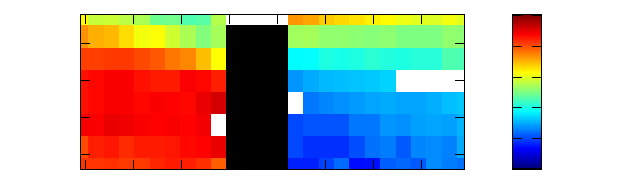
\includegraphics{images/bands4}}%
    \gplfronttext
  \end{picture}%
\endgroup
